\newpage{\cleardoublepage}
\chapter{Marco te\'{o}rico}

\section{Factor de potencia y distorsión de la onda.}

Las distorsiones presentes en la onda se interpreta como un ruido eléctrico. Estas distorsiones es la sobre posición de señales en múltiplos de la frecuencia fundamental. Los armónicos se encuentran en equipos principales generadores de armónicos que efectúan circuitos de rectificación como por ejemplo computadores, televisores, microondas; etc. \cite{A28}\\  Como un caso base, se considera una carga lineal R-L mostrado en \ref{fig:RL} alimentado por medio de una fuente sinusoidal en estado estable. Usando valores rms para las magnitudes de voltaje y corriente, la potencia suministrada por la fuente es:\cite{A29}\\
\begin{equation}\label{EQ1}
P=V_{s}I_{s}cos \phi\\
\end{equation}

El factor de potencia (FP), se conoce como la analogía entre la potencia real media P y el producto de la tensión y corriente rms:
\begin{equation}\label{EQ2}
PF=\frac{P}{V_{s}I_{s}}=cos\phi\\
$(Usando \ref{EQ1})$  \\
\end{equation} 

Y por lo tanto, la corriente rms es:\\

\begin{equation}\label{EQ3}
I=\frac{P}{V_{s}PF}\\
$(Usando \ref{EQ2})$  \\
\end{equation} 

Esto demuestra que el PF y la corriente $I_{s}$ son inversamente proporcional. \\

\begin{figure}[H]
\centering
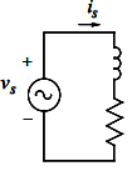
\includegraphics{2Marco/CargaRL}
\caption{ Circuito RL  } 
\label{fig:RL}
\end{figure} 


%\begin{equation}\label{eq1}
%E_{c}=\frac{1}{2}m v^2\\
%\end{equation}
%Donde:\\\\
%$E_{c}$: Energía Cinética\\
%$m$: Masa Propia Del Aire\\
%$v$: Velocidad Propia Del Aire.\\


\section{Distorción armónica total (THD) y valor RMS de la corriente distorsionada}


Una señal de corriente sinusoidal para una carga lineal como en \ref{fig:RL}, no tiene distorsión, sin embargo, hay señales de corrientes que su forma de onda es distorsionada, esto se debe a los equipos generadores de armónicos mencionados en el primer indice. \cite{A29} Un ejemplo de una señal con distorsión se puede ver en \ref{fig:distorsion_current} en donde $i_{s}$ es la señal de corriente distorsionada y $V_{s}(t)$ es sinusoidal. El análisis se aplica a la utilidad de suministros ya sean en monofásico o trifásico, en donde el estudio se realiza por fases.\\
  
\begin{figure}[H]
\centering
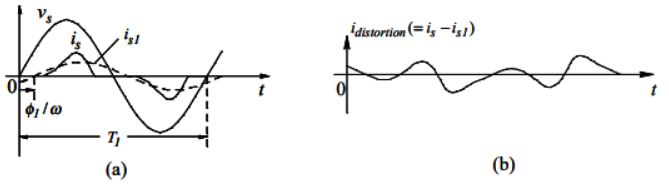
\includegraphics{2Marco/distorsin}
\caption{ Señal de corriente con distorsión (a) Fase de la corriente y su componente fundamental; (b) Componente de distorsión} \cite{A29} 
\label{fig:distorsion_current}
\end{figure} 

La onda periódica de la corriente $i_{s}(t)$, se puede expresar en componentes de Fourier:\\
\begin{equation}\label{EQ4}
i_{s}(t)=i_{s1}(t) + \sum_{h=2}^{\infty}i_{sh(t)}\\
\end{equation}
Donde:\\
$\sum_{h=2}^{\infty}i_{sh(t)} = i_{distorsion}(t)$\\

El componente dc se asume como cero e $i_{s}$ es la componente fundamental mostrada en \ref{fig:distorsion_current}(a). Partiendo de la ecuación \ref{EQ4} la componente de distorsión en la corriente es la diferencia entre $i_{s}(t)$ y su componente de frecuencia fundamental:\cite{A29}\\  
 
\begin{equation}\label{EQ5}
i_{distorsión}(t)=i_{s}(t)-i_{s1}(t)\\
\end{equation}

En una forma de onda con su frecuencia de línea $f_{1}$ y su tiempo de periodo $T_{1}(=\frac{1}{f_{1}})$, los componentes en la expresión de \ref{EQ5} son en los múltiplos de $h$ en la frecuencia fundamental, como por ejemplo, el $3^{er}$ armónico $(h=3)$ está en $180 Hz$ con un sistema de $60 Hz$.\cite{A29}\\

Un concepto básico que se usa es que en una forma de onda repetitiva, la integral de el producto de dos componentes armónicos (incluyendo la fundamental) en frecuencias desiguales sobre repeticiones del tiempo de periodo es igual a cero: \cite{A29}\\

\begin{equation}\label{EQ6}
\int_{T_{1}}^{}f_{h1}(t) \cdot g_{h2}(t) \cdot dt = 0\\
\end{equation}
Donde:\\
$h1 \neq h2$\\

Con el fin de obtener el valor rms de $i_{s}(t)$ en \ref{fig:distorsion_current}(a), se aplica el concepto básico de rms:\\

\begin{equation}\label{EQ7}
I_{s}=\sqrt{\frac{1}{T_{1}}\int_{T_{1}}^{}(i_{s})^2(t) \cdot dt}\\
\end{equation}


Donde, de \ref{EQ4}\\

\begin{equation}\label{EQ8}
i^2_{s}=(i_{s1}+ (\sum_{h=2}^{\infty}i_{sh})^2 = i^2_{sh} + \sum_{h=2}^{\infty}i^2_{sh(t)} \\ 
$+ productos en términos de frecuencia de cruce$
\end{equation}

Sustituyendo \ref{EQ8} en \ref{EQ7}, con el concepto visto en la \ref{EQ6}, cada integral de las frecuencias cruzadas es igual a cero,

\begin{equation}\label{EQ9}
I_{s} = \sqrt{\frac{1}{T}\int_{T_{1}}^{}i^2_{s1}(t) \cdot dt + \sum_{h=2}^{\infty}\frac{1}{T_{1}}\int_{T1}^{}i^2_{sh}(t)\cdot dt}\\
\end{equation}
Donde:\\
$\frac{1}{T}\int_{T_{1}}^{}i^2_{s1}(t) \cdot dt = I^2_{sh1}$\\\\
$\sum_{h=2}^{\infty}\frac{1}{T_{1}}\int_{T1}^{}i^2_{sh}(t)\cdot dt = I^2_{distorsion}$\\\\
Por lo tanto,\\
\begin{equation}\label{EQ10}
I_{s} = \sqrt{I^2_{s1}+I^2_{distorsion}}\\\\
\end{equation}

Donde los valores rms del componente de la frecuencia fundamental y los componentes de distorsión son los siguientes:\\
\begin{equation}\label{EQ11}
I_{s1}=\sqrt{\frac{1}{T}\int_{T1}^{}i^2_{s1}(t) \cdot dt}\\
\end{equation}
y\\
\begin{equation}\label{EQ12}
I_{distorsion}=\sqrt{\sum_{h=2}^{\infty}\left(\frac{1}{T_{1}}\int_{T_{1}}^{}i^2_{sh}(t)\cdot dt\right)}=\sqrt{\sum_{h=2}^{}I^2_{sh}}\\\\
\end{equation}

La ecuación descrita anteriormente, presenta que el valor rms de la componente de distorsión en \ref{fig:distorsion_current} puede ser obtenido de s valores de las componentes individual de los armónicos.\cite{A29}\\

Tomando como referencia los valores rms de los componentes de la distorsión y la fundamental en la corriente $i_{s}(t)$, un indice de distorsión llamado Distorsión Armónica Total (THD) es definida en porcentaje y este mismo pude ser presentado en distintas formas bajo las siguientes ecuaciones:\\

\begin{equation}\label{EQ13}
\%THD = 100*\frac{I_{distorsion}}{I_{s1}}\\
=100*\frac{\sqrt{I^2_{s}-I^2_{s1}}}{I_{s1}}\\
=100*\frac{\sqrt{\sum_{h=2}^{\infty}I^2_{sh}}}{I_{s1}}\\
\end{equation}



\section{ Definiciones del STD IEEE 1459 para la medición de calidad energética bajo condiciones balanceadas y des balanceadas }
\subsection{Mono-fase}
\subsubsection{Mono-fase sinusoidal}

Se parte de una entrada de tipo sinusoidal:\\
\begin{equation}\label{EQ14}
v=\sqrt{2}V sin(\omega t)\\
\end{equation}

Y si a esta, se le conecta una carga lineal, se producirá una corriente sinusoidal de tipo:\\

\begin{equation}\label{EQ15}
i\sqrt{2}I sin(\omega t - \theta)\\
\end{equation}

Donde:\\
$V$ es el valor rms de el voltaje $(V)$\\
$I$ es el valor rms de el voltaje $(I)$\\
$\omega$ es la frecuencia angular  $2\pi f(rad/s)$\\
$f$ es la frecuencia del sistema $(Hz)$\\
$\theta$ es el ángulo de fase entre el voltaje y la corriente  $(rad)$\\
$t$ es el tiempo $(s)$\\
\subsubsection{Potencia activa(W)}

La potencia activa P o también conocida como potencia real, es la medición del flujo de energía durante in intervalo de tiempo $\tau$ a $\tau + KT$. \cite{A30}\\

\begin{equation}\label{EQ16}
P=\frac{1}{KT}\int_{\tau}^{\tau + KT}pdt = \frac{1}{KT}\int_{\tau}^{\tau + KT}p_{a}dt\\
\end{equation}

Donde:\\
$T=1/f$ es el ciclo de tiempo $(s)$\\
$k$     es un número entero positivo $(s)$\\
$\tau$  es el momento cuando empieza la medición $(s)$\\
$P=VIcos \theta$\\
\subsubsection{Potencia Reactiva (var)}

La magnitud de la potencia reactiva $Q$ iguala la amplitud de la potencia reactiva instantánea $P_{q}$.\cite{A30}\\
\begin{equation}\label{EQ17}
Q=VIsin \theta\\
\end{equation}
\begin{equation}\label{EQ18}
Q=\frac{\omega}{KT}\int_{\tau}^{\tau + KT}i\left[\int_{}^{}vdt\right] dt\\
\end{equation}

Sí la carga es inductiva, entonces $Q>0$. Sí la carga es capacitiva, entonces $Q<0$. Por lo tanto, cuando la corriente atrasa el voltaje $\theta>0$ y viceversa.\\
\subsubsection{Potencia Aparente (VA)}

La potencia aparente $S$ es el producto del voltaje rms y corriente rms.\cite{A30}\\

\begin{equation}\label{EQ19}
S=VI
\end{equation}

$S=\sqrt{P^2+Q^2}$ \\

La potencia aparente de una carga monofásica se puede interpretar como la potencia activa total que se puede transmitir a través de la misma línea mientras se mantiene el voltaje rms constante de la carga y a línea de alimentación  de pérdida de potencia constante.\cite{A30}\\

\subsubsection{Factor de potencia}

\begin{equation}\label{EQ20}
PF=\frac{P}{S}
\end{equation}

El factor de potencia se puede interpretar como el radio entre la energía transmitida a la carga sobre la energía máxima que podría transmitirse, siempre y cuando las pérdidas de línea se mantengan iguales.\cite{A30}\\

Para un $S$ y $V$ dados, la utilización máxima de la línea es obtenida cuando $P=S$, por lo tanto, el radio $P/S$ es un indicador de factor de utilización.\cite{A30}\\
 \subsubsection{Potencia Compleja (VA)}
 
 La potencia compleja es una cantidad la cual la potencia activa es la parte real y la potencia reactica es la parte imaginaría.\cite{A30}\\
 
 \begin{equation}\label{EQ21}
 S = P+jQ =  VI^*\\
\end{equation}  

Esta expresión proviene del triángulo de potencias $S,P$ Y $Q$. En la figura \ref{fig:triangulo} se observa un resumen de las direcciones del flujo de potencia. El ángulo $\theta$ es el ángulo de fase de la impedancia equivalente compleja $Z/ \theta = \textbf{V/I}$.\cite{A30}\\ 

\begin{figure}[H]
\centering
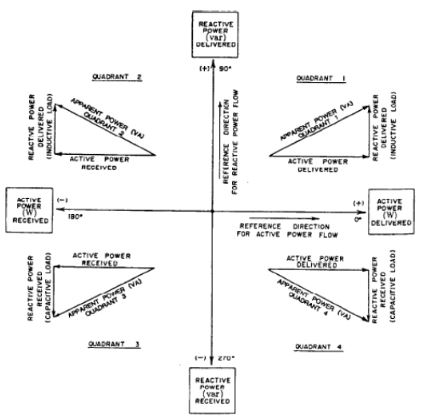
\includegraphics{2Marco/triangulopotencias}
\caption{ Cuatro cuadrantes de las direcciones del flujo de potencia} \cite{A30} 
\label{fig:triangulo}
\end{figure} 


\subsection{Mono-fase no sinusoidal}

Para condiciones estables, una señal de corriente o voltaje no sinusoidal periódica, tiene dos componentes distintos: Los componentes del sistema de frecuencia $V_{1}$ e $i_{1}$ y el termino restante $v_{H}$ e $i_{H}$.\cite{A30}\\

\begin{equation}\label{EQ22}
v=v_{1}+v_{H} 
\end{equation}
e\\\\
$i=i_{1}+i_{H}$\\\\
Donde:\\\\
$v_{1}=\sqrt{2V_{1}}sin(\omega t - \alpha_{1})$\\\\
$i_{1}=\sqrt{2I_{1}}sin(\omega t - \beta_{1})$\\\\
$v_{H}=V_{0}+\sqrt{2}\sum_{h\neq 1}^{}V_{h}sin(h\omega t-\alpha_{h})$\\\\
$i_{H}=I_{0}+\sqrt{2}\sum_{h\neq 1}^{}I_{h}sin(h\omega t-\beta_{h})$\\\\

Las formas de ondas distorsionadas de a menudo contienen componentes de frecuencias llamadas armónicos. Un grupo especial de inter-armónicos es caracterizado por $h<1$. Estos armónicos tienen periodos más largos que el periodo $T$ de la frecuencia fundamental.\cite{A30}\\

Si la onda de corriente o voltaje distorsionada está compuesta únicamente, la medición en intervalos de tiempo $kT$, no permitirá una medición correcta de rms y valores de potencia. \cite{A30}\\

Si al menos uno de los inter-armónicos de orden $h$ es irracional, la onda observada no es periódica. En tal caso las mediciones deberían ser infinitas con el fin de tener una medición correcta del rms y las potencias.\cite{A30}\\

\subsubsection{Distorsión Total Armónica (THD) } 

La desviación en general de una onda distorsionada, se puede estimar con la ayuda de la distorsión armónica total. La distorsión armónica total del voltaje es el siguiente:\\

\begin{equation}\label{EQ23}
THD_{v}=\frac{V_{H}}{V_{1}}=\sqrt{\left(\frac{V}{V_{1}}\right)^2-1}\\
\end{equation}

La distorsión armónica total de corriente es el siguiente:\\
\begin{equation}\label{EQ24}
THD_{I}=\frac{I_{H}}{I_{1}}=\sqrt{\left(\frac{I}{I_{1}}\right)^2-1}\\
\end{equation}

\subsubsection{Potencia Activa (W)}

\begin{equation}\label{EQ25}
P=\frac{1}{kT}\int_{\tau}^{\tau + kT}pdt=\int_{\tau}^{\tau + kT}p_{a}dt\\
\end{equation}
$P=P_{1}+P_{H}$\\

\subsubsection{Potencia activa fundamental (W)}


\begin{equation}\label{EQ26}
P_{1}=\frac{1}{kT}\int_{\tau}^{\tau + kT}v_{1}i_{1}dt=V_{i}I_{1}cos \theta_{1}
\end{equation}

\subsubsection{Potencia Aparente (VA)}

\begin{equation}\label{EQ27}
S=VI\\
\end{equation}

La potencia aparente es la cantidad de potencia activa que pueden ser suministradas a la carga en condiciones ideales.\cite{A30}\\

\subsubsection{Potencia aparente fundamental (VA)}

La potencia fundamental $S_{1}$ y sus componentes $P_{1}$ y $Q_{1}$ son las cantidades actuales que ayudan a definir el tipo de flujo del campo magnético asociado con el voltaje y la corriente fundamental.\cite{A30}\\

\begin{equation}\label{EQ28}
S_{1}=V_{1}I{1}
\end{equation}

\subsubsection{Potencia Aparente no fundamental}

\begin{equation}\label{EQ29}
S_{N}=\sqrt{S^2-S^2_{1}}
\end{equation}

También se puede expresar mediante la siguiente ecuación:

\begin{equation}\label{EQ30}
S^2_{N}=D^2_{I}+D^2_{V}+S^2_{H}\\
\end{equation}

Donde\\

$D_{1}=V_{1}I_{H}=S_{1}(THD_{I})$           Es la potencia de corriente de distorsión (var).\\
$D_{v}=V_{H}I_{1}=S_{1}(THD_{V})$           Es la potencia de voltaje de distorsión (var).\\
$S_{H}=V_{H}I_{H}=S_{1}(THD_{I})(THD_{V})$  Es la potencia de corriente de distorsión (VA).\\

\subsubsection{Potencia de distorsión armónica (var)}

\begin{equation}\label{EQ31}
D_{H}=\sqrt{S^2_{H}-P^2{H}}\\
\end{equation}

\subsubsection{Potencia no activa (var)}

\begin{equation}\label{EQ32}
N=\sqrt{S^2-P^2}\\
\end{equation}

Esta potencia agrupa componentes no activas fundamentales y no fundamentales.\cite{A30}\\

\subsubsection{Factor de potencia fundamental}

\begin{equation}
P_{F1}=cos \theta_{1} = \frac{P_{1}}{S_{1}}\\
\end{equation}

Este radio, facilita la evaluación de las condiciones del flujo energía.\cite{A30}\\

\subsubsection{Factor de potencia}


\begin{equation}\label{EQ33}
PF=\frac{P}{S}
\end{equation}

Dados un $S$ y un $V$, la máxima utilización de la línea es obtenido cuando $P=S$, por lo tanto, el radio $P/S$ es un indicador de factor de utilización.\cite{A30}\\

Cuando el $THD_{v}<5\%$ y $THD_{i}>40\%$, es conveniente usar la siguiente ecuación:\\

\begin{equation}\label{EQ34}
PF=\frac{1}{\sqrt{1+THD^2_{I}}}PF_{1}\\
\end{equation}



\subsection{Sistema trifásico sinusoidal balanceado }

Para este caso se asume un sistema de secuencia positiva rotativa en sentido anti-horario, a, b, c, lo voltaje linea a neutro son los siguientes:

\begin{equation}\label{EQ35}
v_{a}=\sqrt{2}V sin(\omega t)\\
\end{equation} 
$v_{b}=\sqrt{2}V sin(\omega t-120^{\circ})$\\
$v_{c}=\sqrt{2}V sin(\omega t+120^{\circ})$\\

Las líneas de corriente tienen ecuaciones similares, las cuales son:

\begin{equation}\label{EQ36}
i_{a}=\sqrt{2}I sin(\omega t-\theta)\\
\end{equation} 
$i_{b}=\sqrt{2}I sin(\omega t-\theta -120^{\circ})$\\
$i_{c}=\sqrt{2}I sin(\omega t-\theta +120^{\circ})$\\

En sistemas trifásicos balanceados y perfectamente sinusoidal, los sistemas de bajo voltaje no son comunes, solo bajo condiciones de laboratorio en donde se usan amplificadores de potencia de baja distorsión.\cite{A30}\\

En el caso de un sistemas de tres líneas, con voltajes línea a neutro son definidas asumiendo un nodo neutral artificial, el cual se obtienen con ayuda de tres resistencias idénticas conectadas en \textbf{Y}.

\subsubsection{Potencia activa (w)} 
\begin{equation}\label{Eq37}
P=\frac{1}{kT}\int_{\tau}^{\tau +kT}pdt\\
\end{equation}
$P=3VI\cos\theta=\sqrt{3}V_{\ell \ell}I\cos\theta$\\
Donde\\
$V$              es el voltaje rms de línea a neutro\\
$V_{\ell \ell}$  es el voltaje rms línea a línea\\

\subsubsection{Potencia reactiva}


\begin{equation}\label{EQ38}
Q=3VI\sin\theta=\sqrt{3}V_{\ell \ell}I\sin\theta\\
\end{equation}
$|Q|=\sqrt{S^2-P^2}$\\

\subsubsection{Potencia aparente}

\begin{equation}\label{EQ39}
S=3VI=\sqrt{3}V_{\ell \ell}I\\
\end{equation}

\subsubsection{Factor de potencia}

\begin{equation}\label{EQ40}
PF=\frac{P}{s}\\
\end{equation}

\subsection{Sistema trifásico sinusoidal no balanceada}

En este caso, los tres hilos de corriente \textbf{$I_{a},I_{b}$} y \textbf{$I_{c}$}, no tienen las mismas magnitudes y no están desplazadas exactamente $120^{\circ}$ con respecto una a la otra. Las cargas no balanceadas  conlleva a corrientes asimétricas que a su vez causan asimetría de voltaje. En algunas ocasiones sucede que los tres fasores de voltaje no son simétricos. Esto conduce a corrientes asimétras incluso cuando la carga está perfectamente balanceada.\cite{A30}\\


Las ecuaciones de voltaje línea a neutro son los siguientes:

\begin{equation}\label{EQ41}
v_{a}=\sqrt{2}V_{a}\sin(\omega t+\alpha_{a})\\
\end{equation}
$v_{b}=\sqrt{2}V_{b}\sin(\omega t+\alpha_{b} -120^{\circ})$\\\\
$v_{c}=\sqrt{2}V_{c}\sin(\omega t+\alpha_{c}+120^{\circ})$\\\\
Donde por lo menos una de las tres amplitudes linea a neutro $\sqrt{2}V_{q},\sqrt{2}V_{b},$ o $\sqrt{2}V_{c}$ tiene un valor diferente que al de las otras dos amplitudes. Lo mismo debe aplicar a los ángulos de las fases $\alpha_{a}, \alpha_{b},$ y $\alpha_{c}$. Si un ángulo de fase tiene un valor distinto que los otros dos, el sistema está perdiendo simetría y no es balanceado.\cite{A30}\\


Las ecuaciones de corriente línea a neutro son los siguientes:

\begin{equation}\label{EQ41}
i_{a}=\sqrt{2}I_{a}\sin(\omega t+\beta_{a})\\
\end{equation}
$i_{b}=\sqrt{2}I_{b}\sin(\omega t+\beta_{b} -120^{\circ})$\\\\
$i_{c}=\sqrt{2}i_{c}\sin(\omega t+\beta_{c}+120^{\circ})$\\\\

\subsubsection{Potencia Activa}

\begin{equation}\label{EQ42}
P=\frac{1}{kT}\int_{\tau}^{\tau +kT}pdt\\
\end{equation}
$P=P_{a}+P_{b}+P_{c}$\\\\

Donde $P_{a},P_{b}$ y $P_{c}$ son potencias de fases activas:

\begin{equation}\label{EQ43}
P_{a}=\frac{1}{kT}\int_{\tau}^{\tau +kT}v_{a}i_{a}dt=V_{a}I_{a}\cos\theta_{a};\\ \theta_{a}=\alpha_{a}-\beta_{a}\\
\end{equation}
$P_{b}=\frac{1}{kT}\int_{\tau}^{\tau +kT}v_{b}i_{b}dt=V_{b}I_{b}\cos\theta_{b};$ \hspace{1.5cm} $\theta_{b}=\alpha_{b}-\beta_{b}$\\\\
$P_{c}=\frac{1}{kT}\int_{\tau}^{\tau +kT}v_{c}i_{c}dt=V_{c}I_{c}\cos\theta_{c};$ \hspace{1.5cm} $\theta_{c}=\alpha_{c}-\beta_{c}$\\\\


\subsubsection{Potencias activa en secuencias positivas, negativas y cero (w)}

En sistemas de cuatro hilos, hay situaciones cuando el uso componentes simétricos pueden ser de ayuda. Los componentes simétricos de voltaje $V^{+},V^{-}$ y $V_{0}$ y las componentes de corriente $I^{+},I^{-}$  e $I_{0}$ con sus respectivos ángulos $\theta^{+},\theta^{-}$ y $\theta^{0}$ producen los siguientes tres componentes de potencia activa:\cite{A30}\\

La potencia de secuencia positiva:\\


\begin{equation}\label{EQ44}
P^+=3V^{+}I^{+}\cos\theta^{+}\\
\end{equation} 
La potencia de secuencia negativa:\\


\begin{equation}\label{EQ45}
P^-=3V^{-}I^{-}\cos\theta^{-}\\
\end{equation} 
La potencia de secuencia cero:\\


\begin{equation}\label{EQ46}
P^0=3V^{0}I^{0}\cos\theta^{0}\\
\end{equation} 

La potencia activa total es:

\begin{equation}\label{EQ47}
P=P^{+}+P^{-}+P^{0}\\
\end{equation}

\subsubsection{Potencia reactiva (var)}

Las potencias reactivas por fase son definidas con la ayuda de las siguientes ecuaciones:

\begin{equation}\label{EQ48}
Q_{a}=\frac{\omega}{kT}\int_{\tau}^{\tau +kT}i_{a}\left[\int_{}^{}v_{a}dt\right]dt=V_{a}I_{a}\sin\theta_{a}\\
\end{equation}
$Q_{b}=\frac{\omega}{kT}\int_{\tau}^{\tau +kT}i_{b}\left[\int_{}^{}v_{b}dt\right]dt=V_{b}I_{b}\sin\theta_{b}$\\\\

$Q_{c}=\frac{\omega}{kT}\int_{\tau}^{\tau +kT}i_{c}\left[\int_{}^{}v_{c}dt\right]dt=V_{c}I_{c}\sin\theta_{c}$\\\\

La potencia reactiva total es:\\

\begin{equation}\label{EQ50}
Q=Q_{a}+Q_{a}+Q_{c}\\
\end{equation}

\subsubsection{Potencias aparentes en fase}

\begin{equation}\label{EQ51}
S_{a}=V_{a}I_{a}; \hspace{1cm} S_{b}=V_{b}I_{b}; \hspace{1cm} S_{c}=V_{c}I_{c}\\
\end{equation}
$S^2_{a}=P^2_{a}Q^2_{a};$ \hspace{1cm} $S^2_{b}=P^2_{b}Q^2_{b};$ \hspace{1cm} $S^2_{c}=P^2_{c}I_{c}$\\

\subsubsection{Potencia aparente aritmética }

\begin{equation}\label{EQ52}
S_{A}=S_{a}+S_{b}+S_{c}\\
\end{equation}

$S_{A} \neq \sqrt{P^2+Q^2}$

\subsubsection{Potencia aparente del vector}

\begin{equation}\label{EQ53}
S_{V}=\sqrt{P^2+Q^2}\\
\end{equation}

En la Fig \ref{fig:inter}, se muestra un interpretación de $S_{V}$ y $S_{A}$.

\begin{figure}[H]
\centering
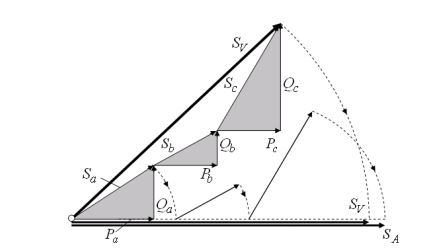
\includegraphics{2Marco/intergeo}
\caption{Potencias aparentes aritmpeticas y de vector} 
\label{fig:inter}
\end{figure} 

\subsubsection{Factor de potencia aritmético y del vector }

\begin{equation}\label{EQ54}
PF_{V}=\frac{P}{S_{V}}\\
\end{equation}
$PF_{A}=\frac{P}{S_{A}}$\\

Una línea trifásica que abastece a uno o más clientes debería ser vista como un solo camino, una entidad que transmite la energía eléctrica a lugares donde es convertida en otras forma de energía. Esta mal ver cada fase como una ruta de energía independiente.\cite{A30}\\

\subsubsection{Potencia aparente efectiva}

Este concepto asume un circuito balanceado virtual que tiene exactamente las mismas líneas de perdidas como el circuito des balanceado actual. Para un sistema de 4 líneas, el balance de la perdida de potencia es expresado en la siguiente ecuación:\cite{A30}\\

\begin{equation}\label{EQ55}
r(I^2_{a}+I^2_{b}+I^2_{c}+\rho I^2_{n})=3rI^2_{e}\\
\end{equation}
Donde:\\\\
$r$			es la resistencia\\
$I_{n}$		es la corriente actual (rms)\\
$r_{n}$		Es el cable neutro de la resistencia\\

De las ecuaciones anteriores, la corriente equivalente de un sistema de 4 líneas es el siguiente:\\

\begin{equation}\label{EQ56}
I_{e}=\sqrt{\frac{I^2_{a}+I^2_{b}+I^2_{c}+\rho I^2_{n}}{3}}=\sqrt{(I^+)^2+(I^-)^2+(1+3\rho)(I^0)^2}\\
\end{equation}

Y para un sistema de tres hilos donde $I^0=0$\\

\begin{equation}\label{EQ57}
I_{e}=\sqrt{\frac{I^2_{a}+I^2_{b}+I^2_{c}}{3}}=\sqrt{(I^+)^2+(I^-)^2}\\
\end{equation}

\subsubsection{Factor de potencia efectiva}

\begin{equation}\label{EQ58}
PF_{e}=\frac{P}{S_{e}}\\
\end{equation}
